\section{Covariance, derivatives and Fisher forecasts}
\label{sec:framework}
% =====================================================================

\paragraph{Data vectors.} By default, the cross-correlations of the extreme quartiles Q1 and Q4 with the galaxies, $\ell=0,2$, $20\le s\le150\Mpch$ in $10\Mpch$ bins (13 bins per multipole, 52 numbers per method), with or without the 2PCF (26 numbers). Variants add the quartile auto-correlations, use the galaxy quartiles, single quartiles, or change the minimum scale.

\subsection{Covariance}

\paragraph{Baseline: 1786 independent boxes.} The covariance is measured on the 1786 official small boxes (Section~\ref{sec:official}): 1786 independent $(500\Mpch)^3$ volumes treated exactly like our subvolumes. Forecasts are quoted for this volume of $0.125\,(h^{-1}{\rm Gpc})^3$. The correlation matrix (Figure~\ref{fig:corr}) shows strong correlations between neighbouring scales, between the Q4 cross-correlations and the 2PCF, and anti-correlations between the Q1 and Q4 blocks. The ASTRA and density-split blocks of the same quartile are very strongly correlated: being measured on the same galaxies, their noise is largely common. This is the origin of their complementarity: when two measurements share most of their noise but respond differently to the parameters, their combination cancels part of that noise and gains much more than independent measurements would.

\paragraph{First approach: 192 subvolumes of one box.} Before the official mocks were used, the covariance was estimated from the fiducial catalogue of the emulator suite (\texttt{c000}, \texttt{hod239}, the c000 draw closest to the centre of the HOD prior), using the 64 subvolumes measured along the three lines of sight, $N_s=192$ samples. The three lines of sight are not independent, an approximation commonly used in simulation-based analyses. The inverse covariance is corrected by the Hartlap factor \cite{Hartlap2007}, $(N_s-N_d-2)/(N_s-1)$: 0.72 for one method ($N_d=52$), 0.59 with the 2PCF ($N_d=78$), 0.31 for ASTRA + DS + 2PCF ($N_d=130$), which motivated the compression of the data vectors (Section~\ref{sec:fishermat}). Section~\ref{sec:choices} shows how replacing this covariance by the independent one changed the comparison.

\begin{figure}[!htbp]
\centering
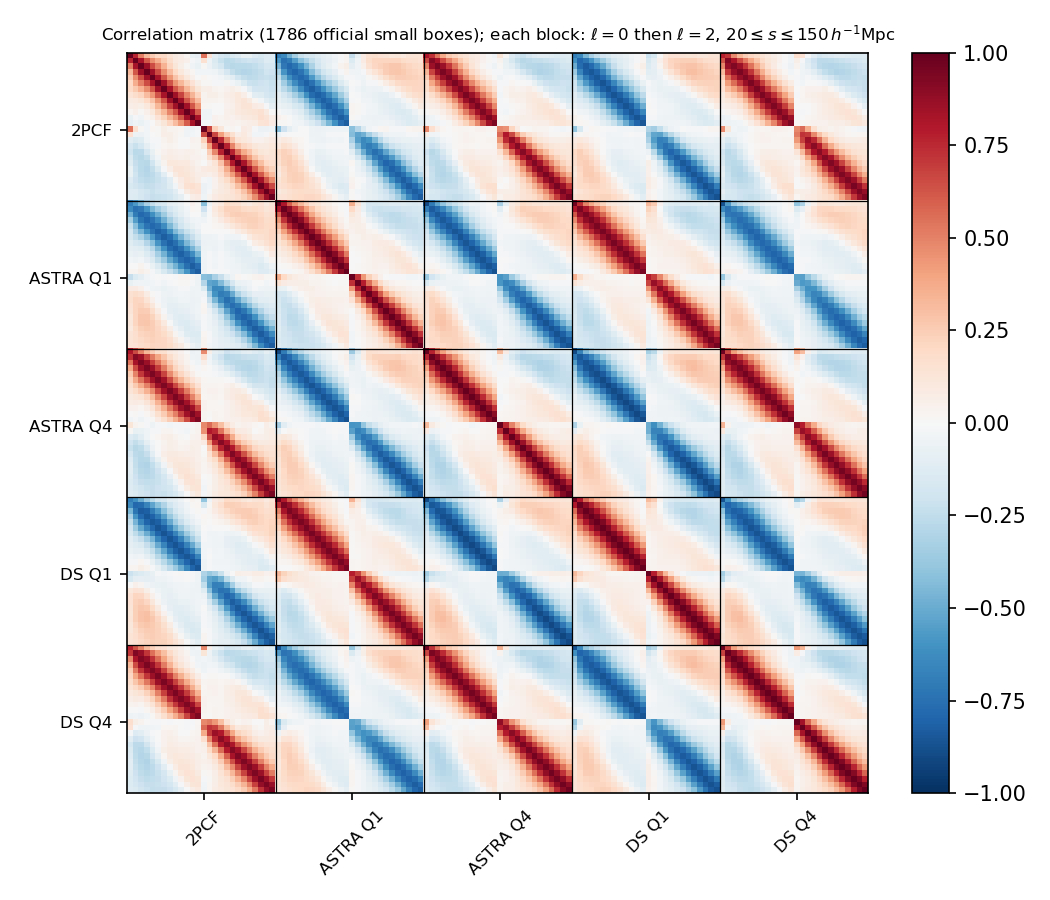
\includegraphics[width=\linewidth]{v2_corr.png}
\caption{Correlation matrix of the 2PCF and of the Q1, Q4 cross-correlations of ASTRA split and density split (1786 official small boxes).}
\label{fig:corr}
\end{figure}

\subsection{Finite differences: the HOD-mismatch problem}
\label{sec:finitediff}

The AbacusSummit derivative grid provides, for each parameter, two simulations differing only by a small change of that parameter and sharing the same initial conditions. A natural estimate of the derivatives is the paired finite difference: for each parameter we select one HOD file in each cosmology of the pair, minimising the distance between the two HOD parameter vectors (Table~\ref{tab:hods}), and difference the statistics subvolume by subvolume and line of sight by line of sight before averaging, so that the cosmic variance common to the two simulations largely cancels. This cancellation is only partial: each HOD catalogue is an independent draw of the galaxies populating the halos, so the galaxy sampling noise is not shared, and the difference of two full-box measurements with different HODs has an error comparable to that of a single box (1.05 times, median over the pairs of the grid). The precision of the paired derivatives comes from the average over the 192 paired samples.

\begin{table}[!htbp]
\centering\small
\begin{tabular}{lccc}
\toprule
Parameter & HOD files & $|\Delta h|$ & random pairs \\
\midrule
fiducial & c000\_hod239 & -- & -- \\
$\omega_b$ & c100\_hod448 / c101\_hod694 & 0.63 & 1.38 \\
$\omega_{\rm cdm}$ & c102\_hod589 / c103\_hod841 & 0.58 & 1.38 \\
$n_s$ & c104\_hod308 / c105\_hod735 & 0.65 & 1.37 \\
$\sigma_8$ & c112\_hod230 / c113\_hod204 & 0.65 & 1.39 \\
\bottomrule
\end{tabular}
\caption{HOD catalogues of the finite-difference pairs. $|\Delta h|$ is the distance between the two HOD parameter vectors normalised to the prior range (12 parameters); the last column gives the median for random pairs.}
\label{tab:hods}
\end{table}

Averaged over the 192 samples, these differences have small statistical errors, but they are not cosmological derivatives: because the HODs of the two cosmologies differ, each difference is dominated by the response to the HOD mismatch, 10--15 times larger than the response to the cosmological parameter. The derivative vectors with respect to $\omega_b$, $n_s$ and $\sigma_8$ are almost collinear (correlations 0.95--0.99 in the Fisher metric) and the Fisher matrices are not positive definite. We tried to calibrate and subtract the HOD response with 72 additional fiducial catalogues spanning the HOD parameters of the pairs: a linear model predicts left-out catalogues with a 45\% error, a Gaussian-process model (one GP per principal component of the data vector, anisotropic kernel) with 8\%. Since the HOD term is an order of magnitude larger than the cosmological one, even 8\% leaves a residual comparable to the signal, and the corrected Fisher matrices remain unstable.

The finite differences are nevertheless not discarded. They (i) diagnose and quantify the limitation of an emulator suite for derivatives, a pitfall generic to suites in which the HOD is sampled independently in each cosmology; (ii) once corrected for the HOD response, provide a check of the emulator derivatives that does not rely on a neural network (Figure~\ref{fig:emu_pairs}); (iii) with several HOD draws per cosmology, become an independent estimator of the derivatives by regression over all the pairs (Section~\ref{sec:regression}).

\subsection{Neural-network emulator}
\label{sec:emulator}

\paragraph{Why an emulator.} As in SUNBIRD \cite{CuestaLazaro2024}, we model each statistic as a smooth function of the cosmological and HOD parameters, and take its derivatives at exactly fixed HOD by automatic differentiation, which removes the HOD mismatch by construction.

\paragraph{Inputs and outputs.} The inputs are the 8 cosmological parameters varied in AbacusSummit ($\omega_b$, $\omega_{\rm cdm}$, $\sigma_8$, $n_s$, $\alpha_s$, $N_{\rm ur}$, $w_0$, $w_a$; $h$ and $A_s$ follow from $\theta_*$ and $\sigma_8$) and the 12 HOD parameters, rescaled to $[0,1]$ over the prior. The output of one network is one statistic, the monopole and quadrupole for $20\le s\le150\Mpch$ in $10\Mpch$ bins (26 numbers), measured on the full box as the mean of the 64 subvolumes, standardised by its mean and by the statistical error of the full box $\sigma_{\rm box}$. There is one network per statistic (33 statistics).

\paragraph{Architecture and training.} Fully-connected networks with three hidden layers of 256 units and SiLU activations, smooth so that their derivatives are well behaved, trained with Adam and early stopping on a validation set. With the standardisation above the loss is a $\chi^2$ per bin. Each statistic has an ensemble of 10 networks with different initialisations; the prediction is the ensemble mean, and the scatter between members measures the uncertainty due to training.

\paragraph{Training set.} 999 catalogues of the 85 cosmologies: 8 HOD draws per cosmology, the 72 fiducial calibration catalogues, and 16 draws close to the fiducial HOD in c000 and in each of the 14 cosmologies of the derivative grid, where the derivatives are evaluated (densification, below). Validation and test sets are 8 cosmologies each, never seen in training.

\paragraph{Accuracy.} On the test cosmologies the emulator reproduces all 33 statistics with a median error of 0.4--0.9 $\sigma_{\rm box}$, about ten times below the error of the $(500\Mpch)^3$ volume of the forecasts (Figure~\ref{fig:emu}); the emulator error is nevertheless added to the covariance. A learning curve, retraining on 25, 50, 75 and 100\% of the training set, shows that this error has reached a plateau at $\simeq0.5\sigma_{\rm box}$, set by the galaxy sampling noise of single catalogues: more catalogues would barely help (Appendix~\ref{app:path}).

\paragraph{Cosmological response.} Accurate predictions do not guarantee accurate derivatives. We test the latter by training the emulator without the 14 cosmologies of the derivative grid and comparing its prediction of the $\pm$ pair differences, HOD mismatch included, to the simulations (Figure~\ref{fig:loco}). The response to $\sigma_8$ and $n_s$ is reproduced to 10--20\%, the response to $\omega_b$ to 30--45\% with the correct shape, but the response to $\omega_{\rm cdm}$ is not captured below $s\simeq70\Mpch$: at fixed $\theta_*$ and $\sigma_8$ its effect is smaller than the emulator error and is not learnt away from the training points. This led us to \emph{densify} the training set around the fiducial point with the 16 HOD draws closest to the fiducial HOD in c000 and in each cosmology of the grid (240 catalogues), so that the emulator sees the response to each parameter for many similar galaxy--halo connections. Densification alone did not stabilise the derivatives: the Fisher errors of the individual networks scattered by 70--170\% for the 2PCF and for $\omega_{\rm cdm}$ and $n_s$, and the ASTRA/density-split comparison changed sign between trainings. As an independent check, the derivatives of the emulator at fixed HOD agree with the GP-corrected pair differences to 1--3\% for $n_s$ and $\omega_{\rm cdm}$, 5--6\% for $\sigma_8$ and 8--13\% for $\omega_b$ (Figure~\ref{fig:emu_pairs}).

\paragraph{Training on catalogue differences.} To constrain the response near the fiducial point directly, we add to the loss the $\chi^2$ of the predicted \emph{differences} between catalogues, over 2544 pairs: all the pairs $(c_+,h_i),(c_-,h_j)$ of the seven $\pm$ pairs of the grid with HODs within one prior range of the fiducial, and pairs of the same cosmology (HOD response); details in Appendix~\ref{app:maths}. The differences are not much more precise than individual measurements, since the galaxy sampling noise is not shared, but the term constrains their \emph{structure}: the network must reproduce how the statistics change between nearby points of parameter space, which is what the derivatives require. We also tested an additional weight $(25\Mpch/s)^\alpha$, $\alpha=1$, on the small scales. We validated the three variants on 56 local catalogues (4 per grid cosmology) excluded from training, by predicting the differences of all the held-out $\pm$ pairs (Table~\ref{tab:local}, Figure~\ref{fig:local}). The difference term halves the error for $\omega_b$ and $\sigma_8$ and reduces it for all parameters but $\omega_{\rm cdm}$, already reproduced to 11\% near the fiducial; the residuals reach the noise level of the measured differences ($\simeq1\sigma_{\rm box}$), so the data do not allow a more stringent test. The small-scale weight brings a marginal additional gain but makes the forecasts that include the quartile auto-correlations unstable, so we use the difference term without it: this is the baseline emulator.

\begin{table}[!htbp]
\centering\small
\begin{tabular}{lccccccc}
\toprule
 & $\omega_b$ & $\omega_{\rm cdm}$ & $n_s$ & $\alpha_s$ & $w_0$ & $w_0,w_a$ & $\sigma_8$ \\
\midrule
no diff. term & 21 & 11 & 35 & 14 & 17 & 17 & 13 \\
diff. term & 10 & 11 & 27 & 10 & 12 & 10 & 7 \\
+ small scales & 8 & 11 & 26 & 9 & 11 & 8 & 7 \\
\bottomrule
\end{tabular}
\caption{Median relative error (\%) of the emulator prediction of the differences between held-out local catalogues of the $\pm$ pairs of the derivative grid, for the three training variants.}
\label{tab:local}
\end{table}

\paragraph{Derivatives.} Figure~\ref{fig:derivs} shows the baseline derivatives of the 2PCF and of the Q1, Q4 cross-correlations in units of the statistical error: the two methods respond very similarly to $\omega_{\rm cdm}$ and $n_s$, mostly through the monopole at $s<75\Mpch$; the Q1 (void) cross-correlations respond with the opposite sign to Q4 and to the 2PCF, which is what breaks degeneracies; $\sigma_8$ acts mostly on the quadrupoles at fixed HOD. Figures~\ref{fig:der_astra} and~\ref{fig:der_ds} show the derivatives of the four quartiles in the layout of the first version: the response is ordered from Q1 to Q4 for $\omega_{\rm cdm}$ and $n_s$, the extreme quartiles responding most; for $\sigma_8$ at fixed HOD the monopole responses are below $1\sigma$ for density split and the information comes from the quadrupoles.

\begin{figure*}[!tp]
\centering
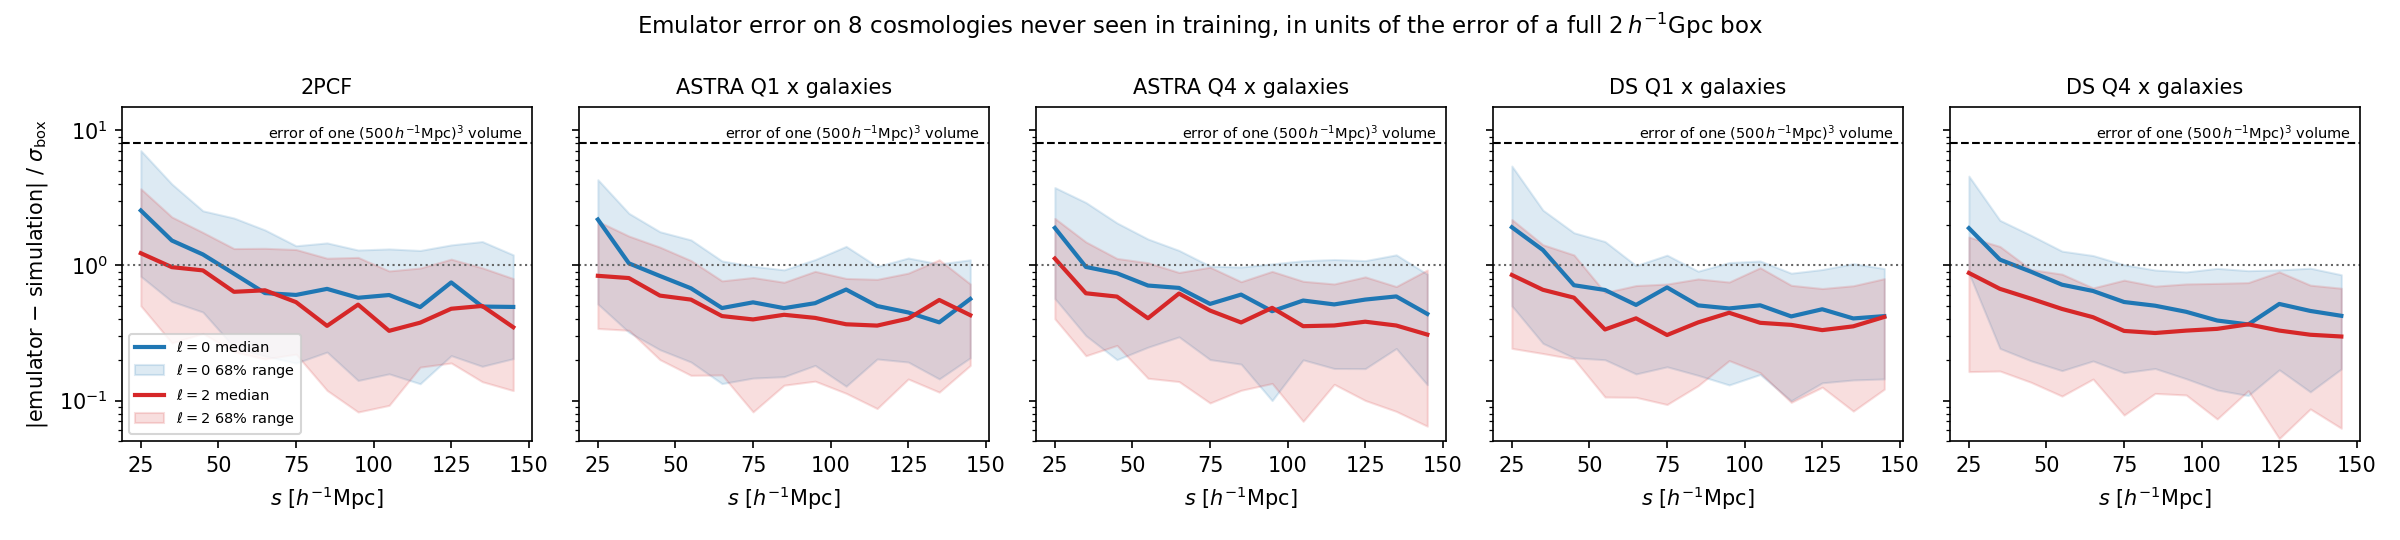
\includegraphics[width=\textwidth]{readable_emulator_validation.png}
\caption{Emulator accuracy on 8 held-out cosmologies (8 HOD draws each): median (lines) and 68\% range (bands) of $|$emulator $-$ simulation$|$ in units of the statistical error of a $2\,h^{-1}$Gpc box, for the monopole (blue) and quadrupole (red) of the 2PCF and of the Q1, Q4 cross-correlations of ASTRA split and density split. Dashed: error of one $(500\Mpch)^3$ volume, the volume of the forecasts.}
\label{fig:emu}
\end{figure*}

\begin{figure*}[!tp]
\centering
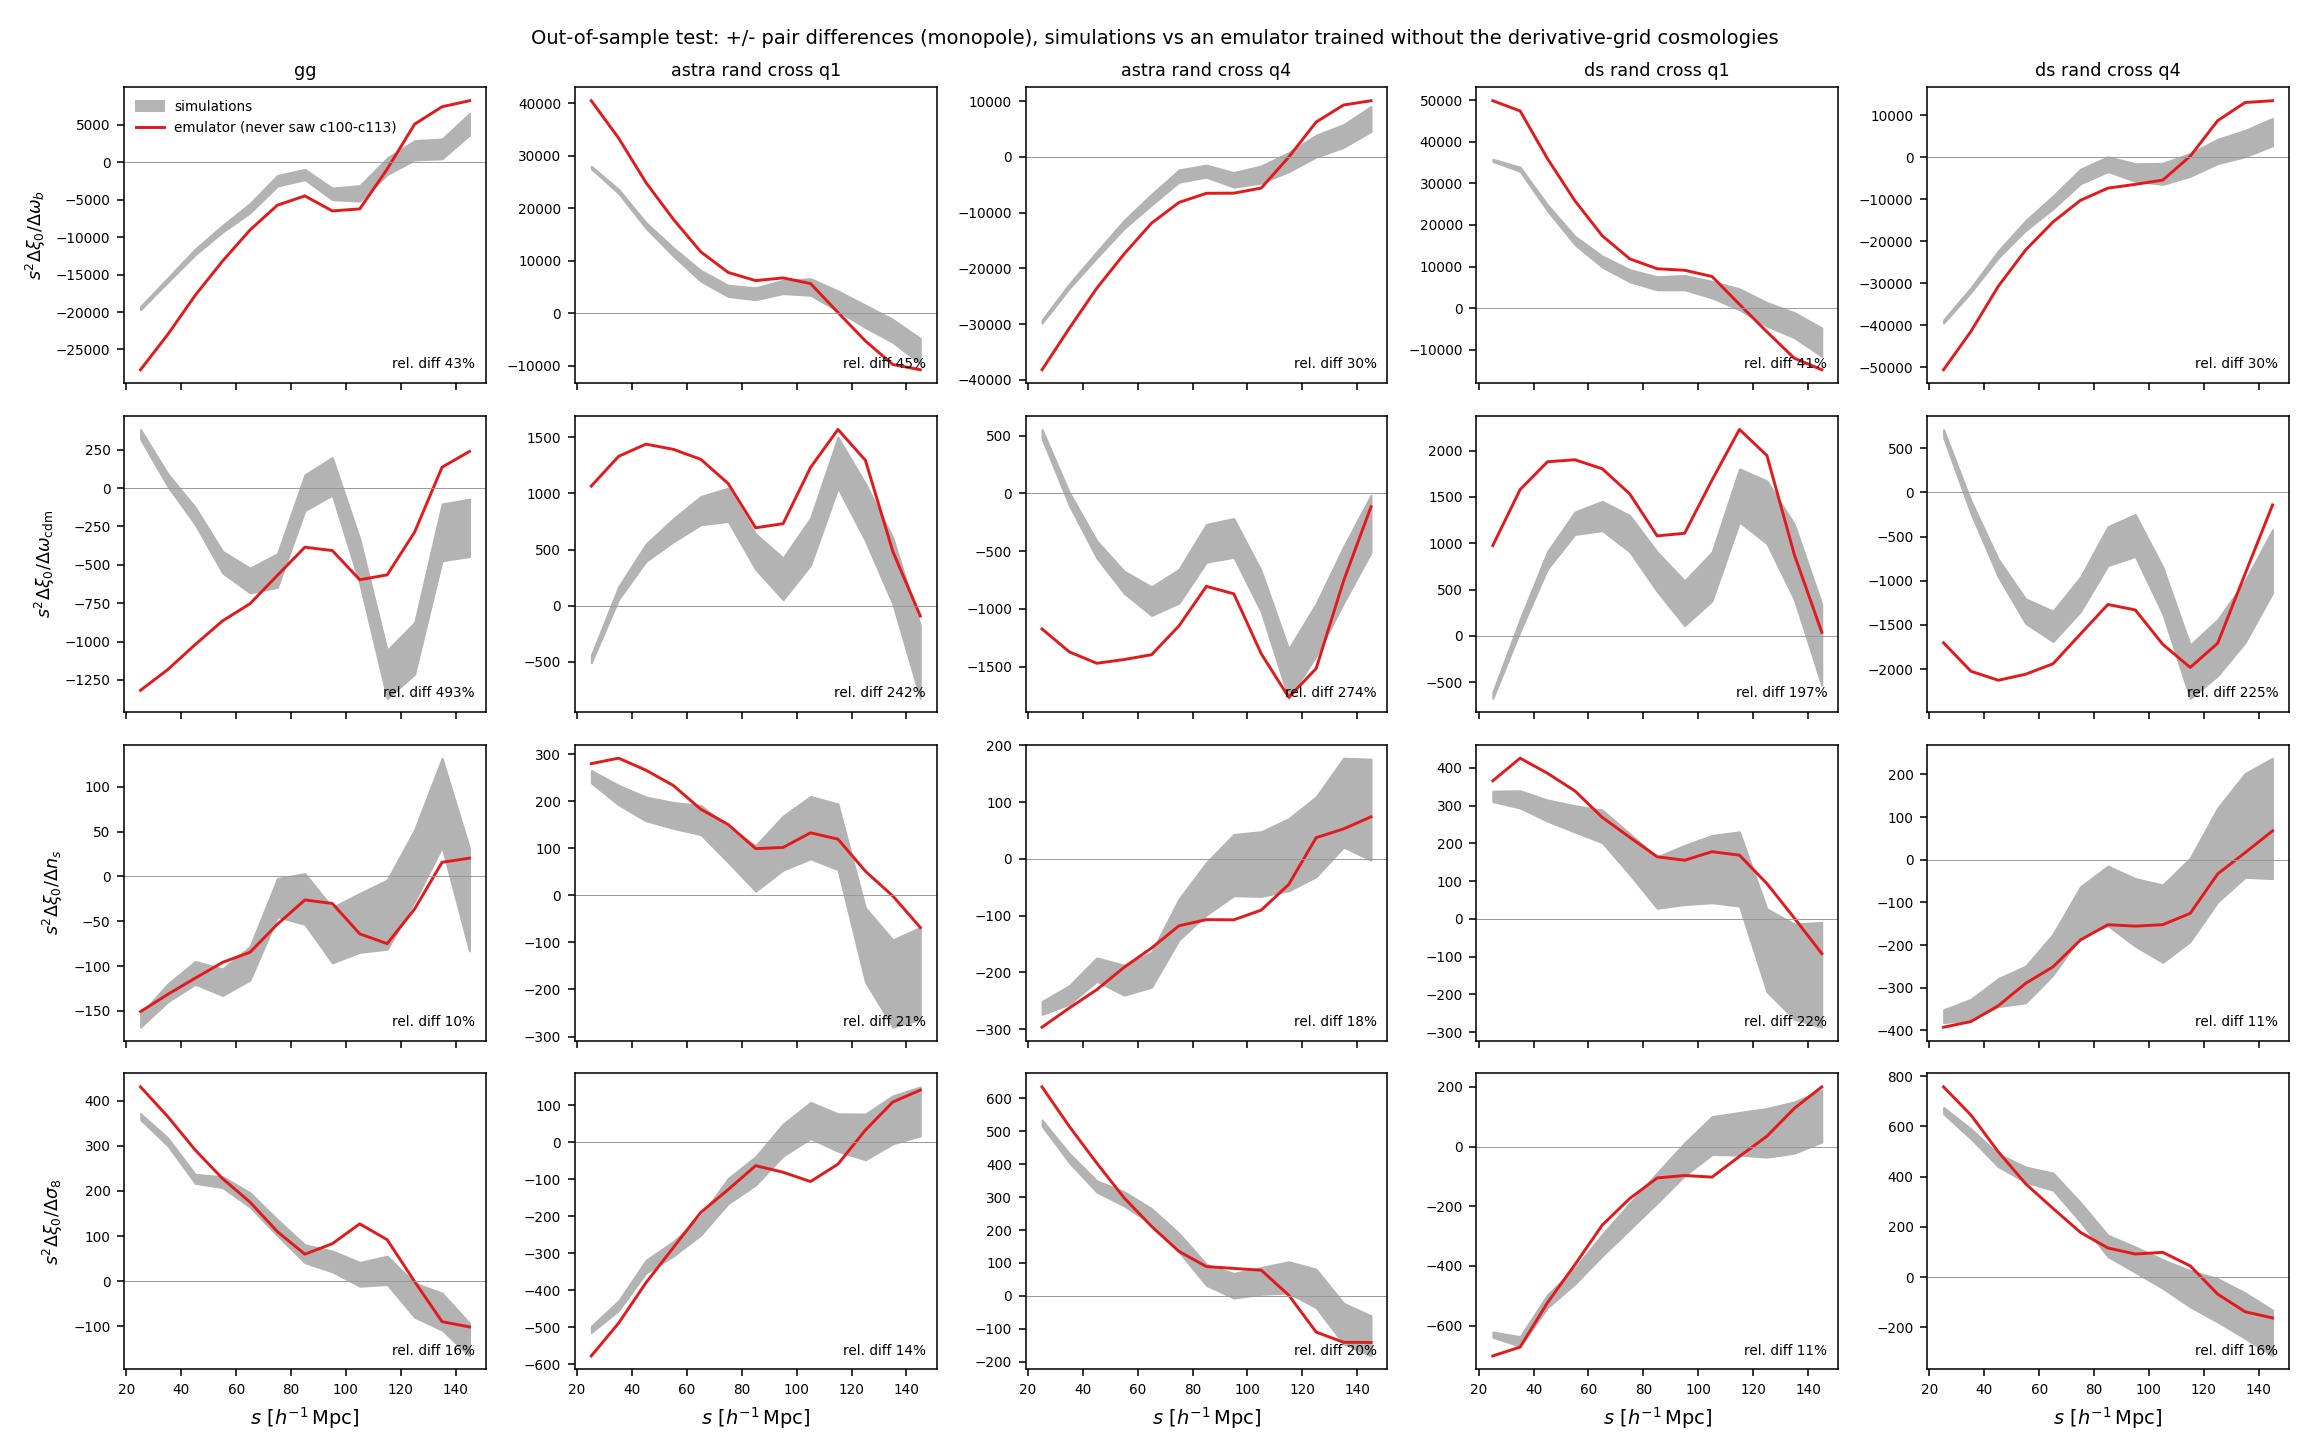
\includegraphics[width=\textwidth]{v2_derivatives_loco.png}
\caption{Out-of-sample test of the cosmological response: monopole of the $\pm$ pair differences in the simulations (grey band: mean $\pm$ error over the 192 paired samples) and predicted by an emulator trained without the cosmologies of the derivative grid (red).}
\label{fig:loco}
\end{figure*}

\begin{figure*}[!tp]
\centering
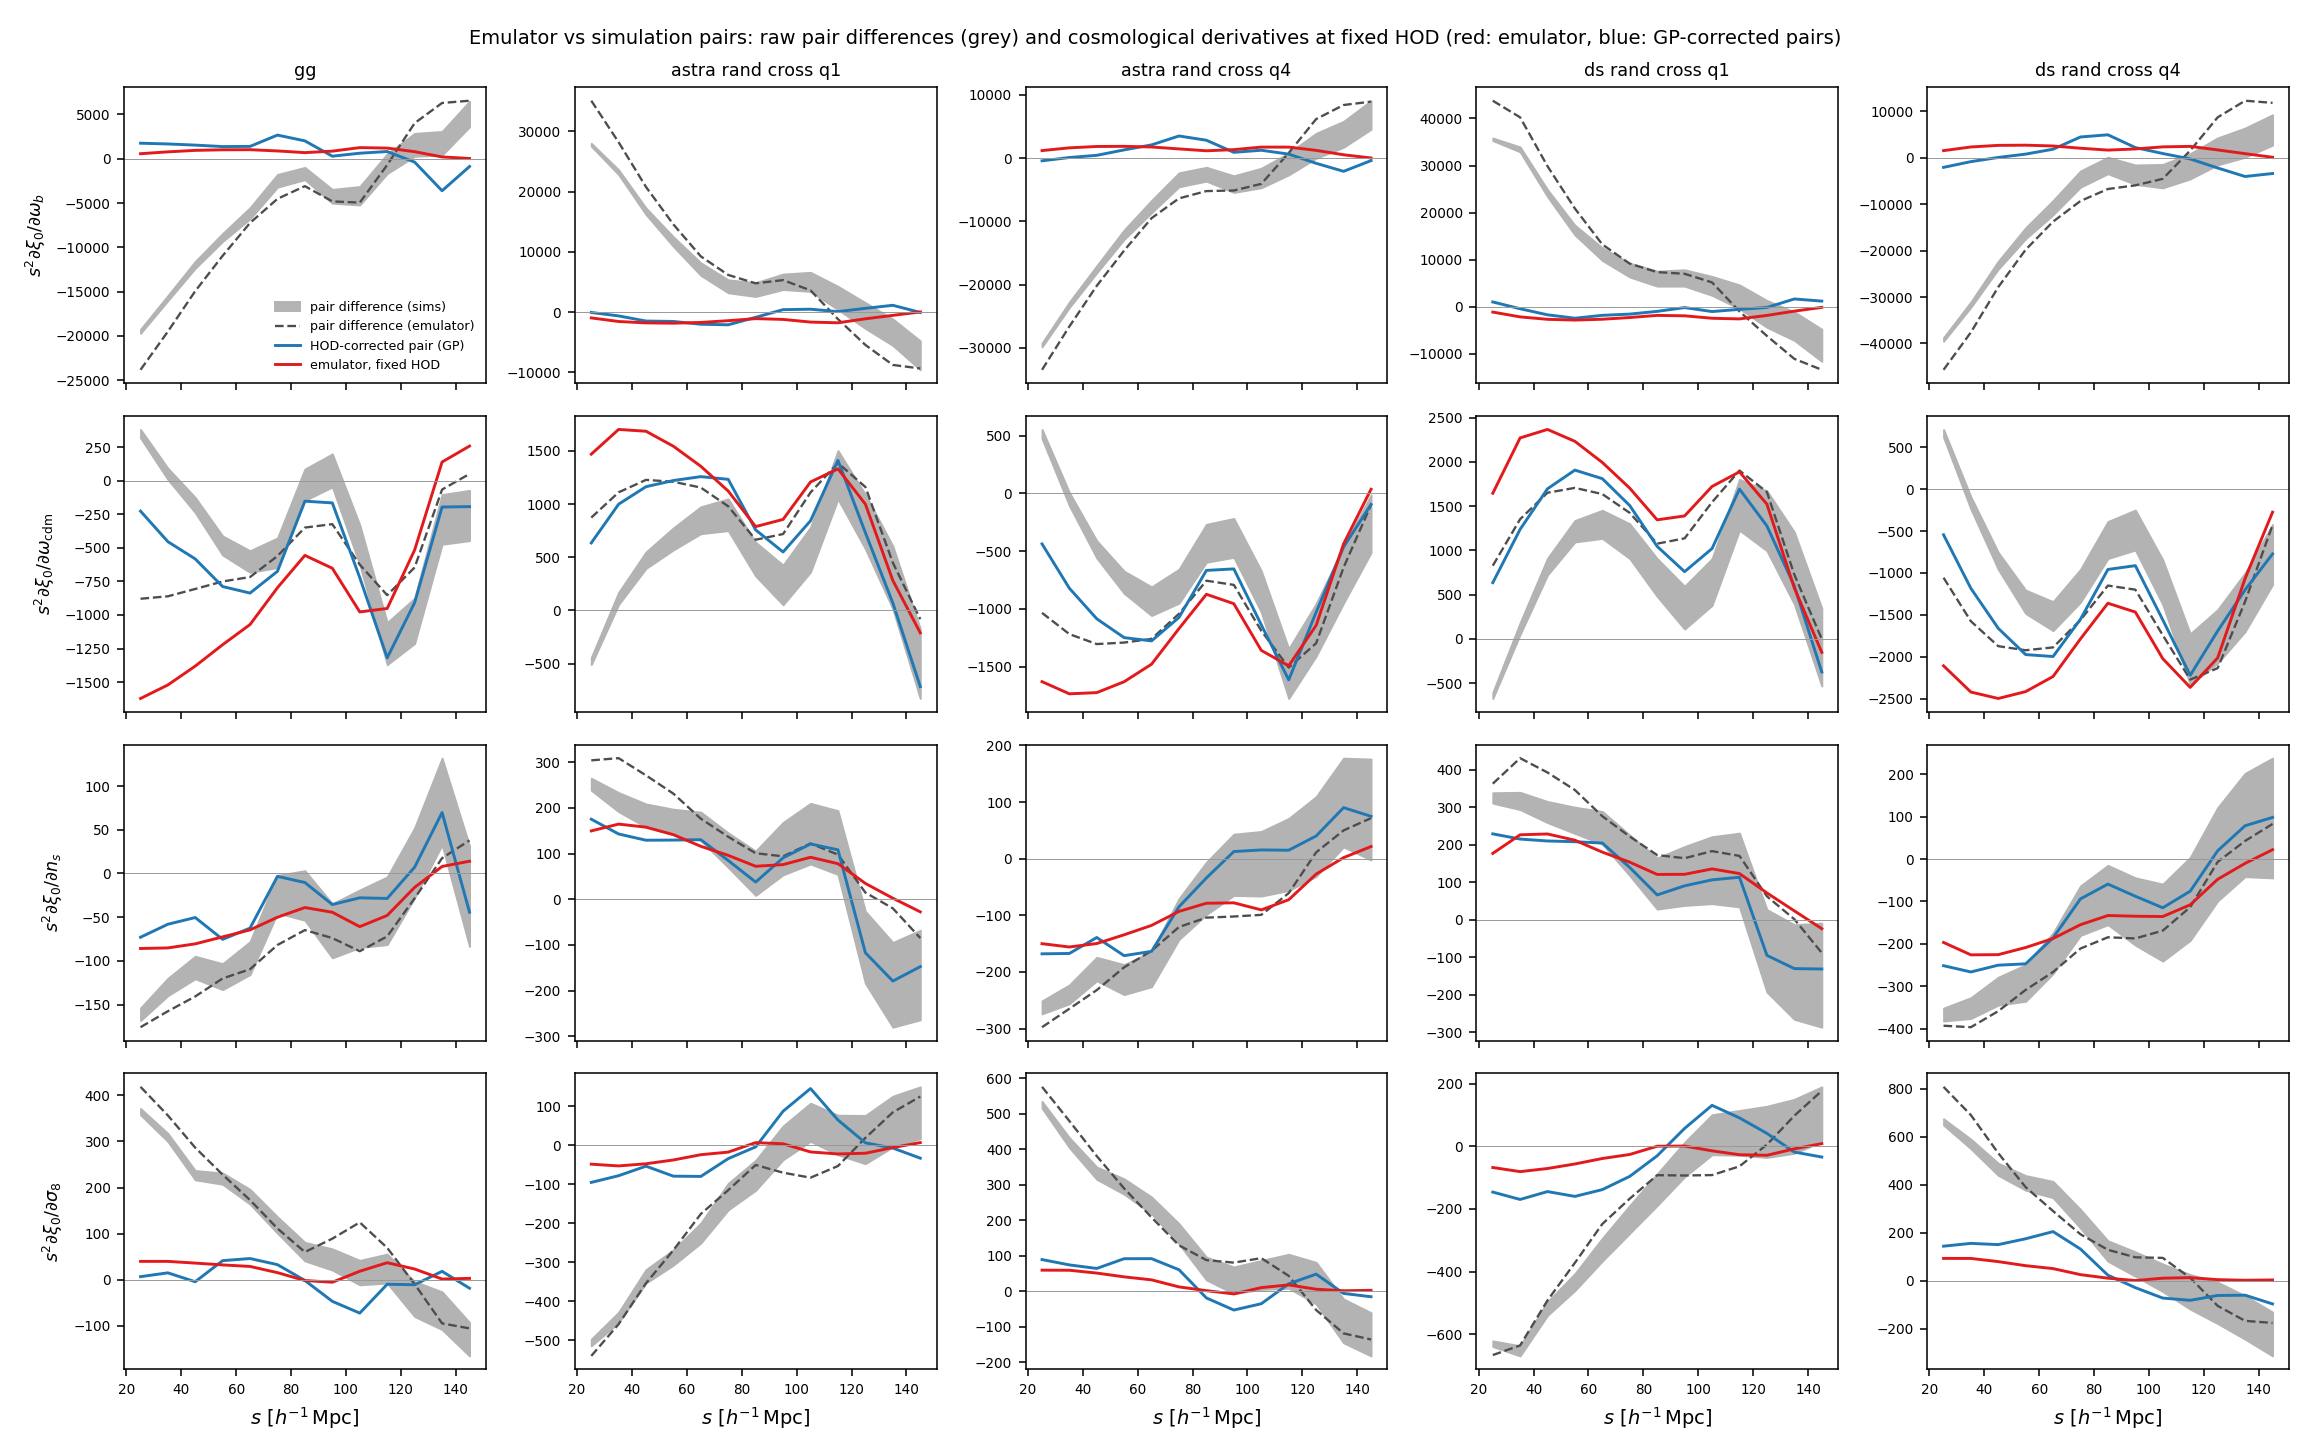
\includegraphics[width=\textwidth]{v2_emulator_vs_pairs.png}
\caption{Cosmological derivatives at fixed HOD from the emulator (red) and from the pair differences corrected with the GP calibration of the HOD response (blue), with the raw pair differences in the simulations (grey) and as predicted by the emulator (dashed).}
\label{fig:emu_pairs}
\end{figure*}

\begin{figure}[!htbp]
\centering
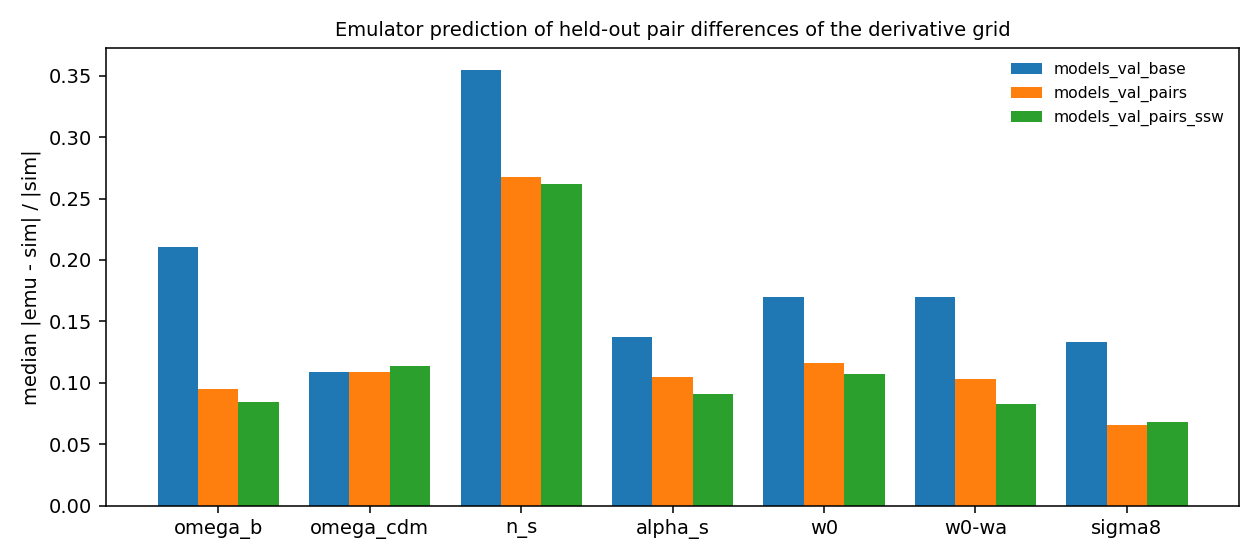
\includegraphics[width=\linewidth]{v2_validate_local.png}
\caption{Median relative error of the emulator prediction of held-out pair differences of the derivative grid, for the three training variants (Table~\ref{tab:local}).}
\label{fig:local}
\end{figure}

\begin{figure*}[!tp]
\centering
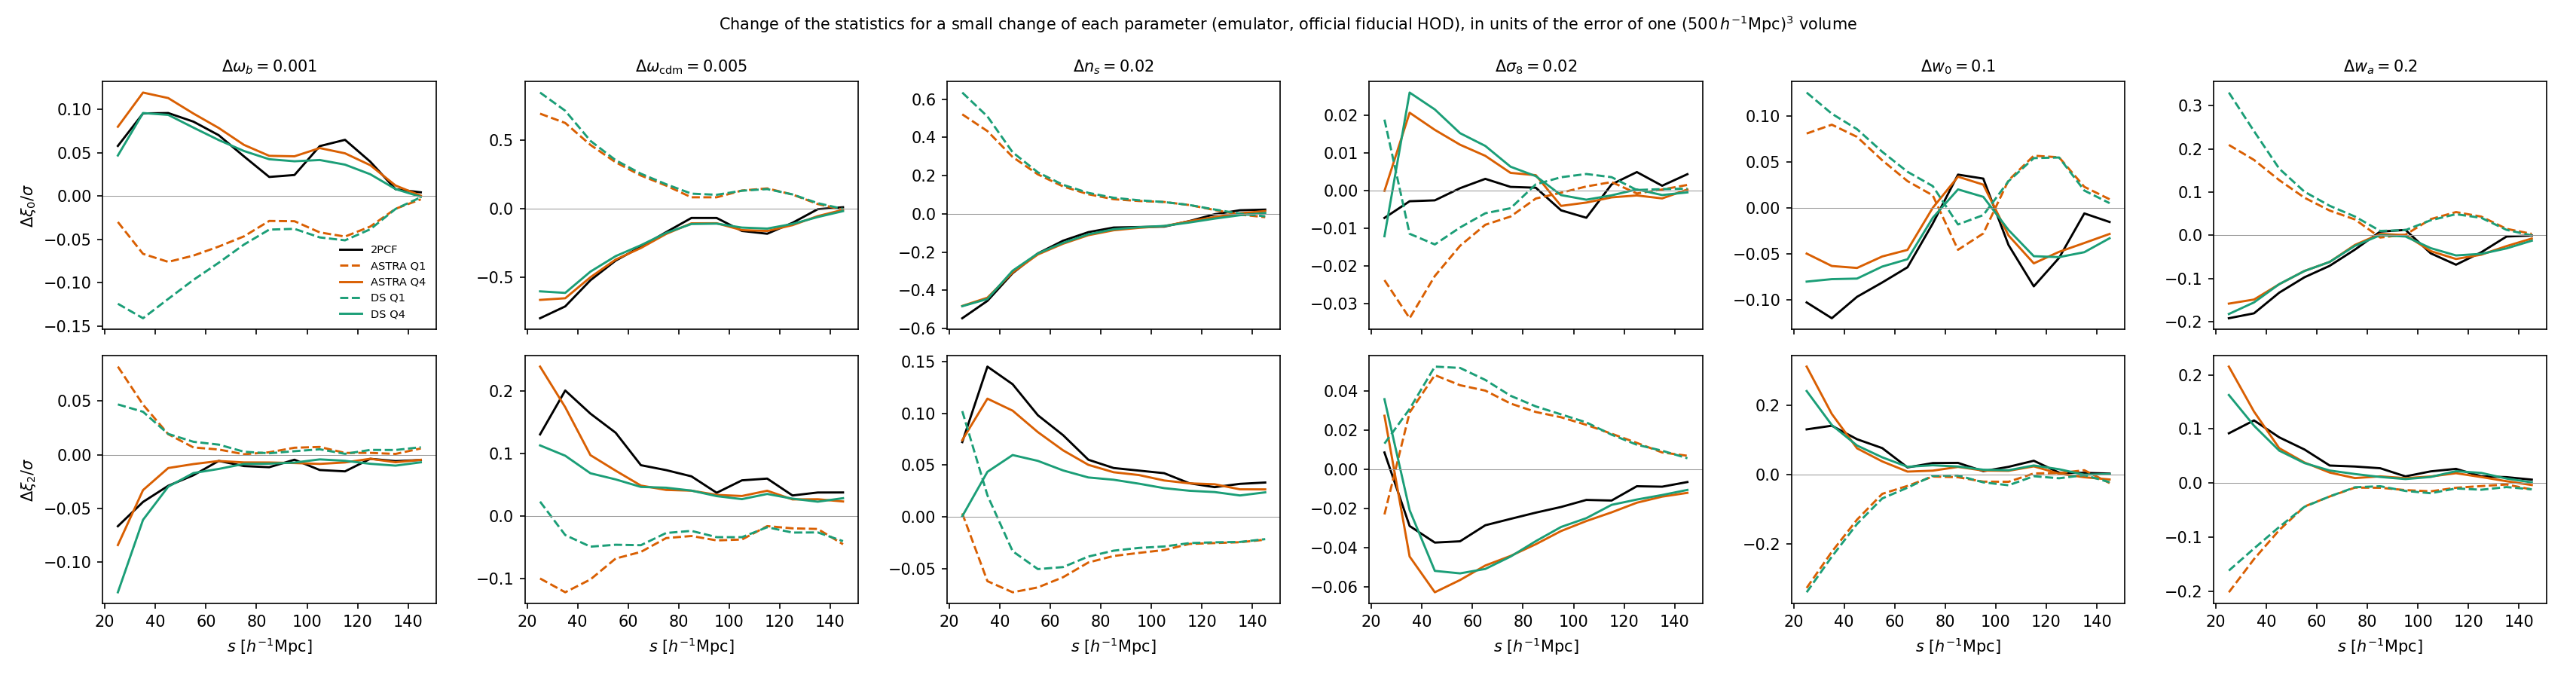
\includegraphics[width=\textwidth]{v2_derivatives.png}
\caption{Change of the monopole (top) and quadrupole (bottom) for a small change of each parameter, in units of the error of one $(500\Mpch)^3$ volume (baseline emulator at the official fiducial point): 2PCF (black), Q1 (dashed) and Q4 (solid) cross-correlations of ASTRA split (orange) and density split (green).}
\label{fig:derivs}
\end{figure*}

\begin{figure}[!htbp]
\centering
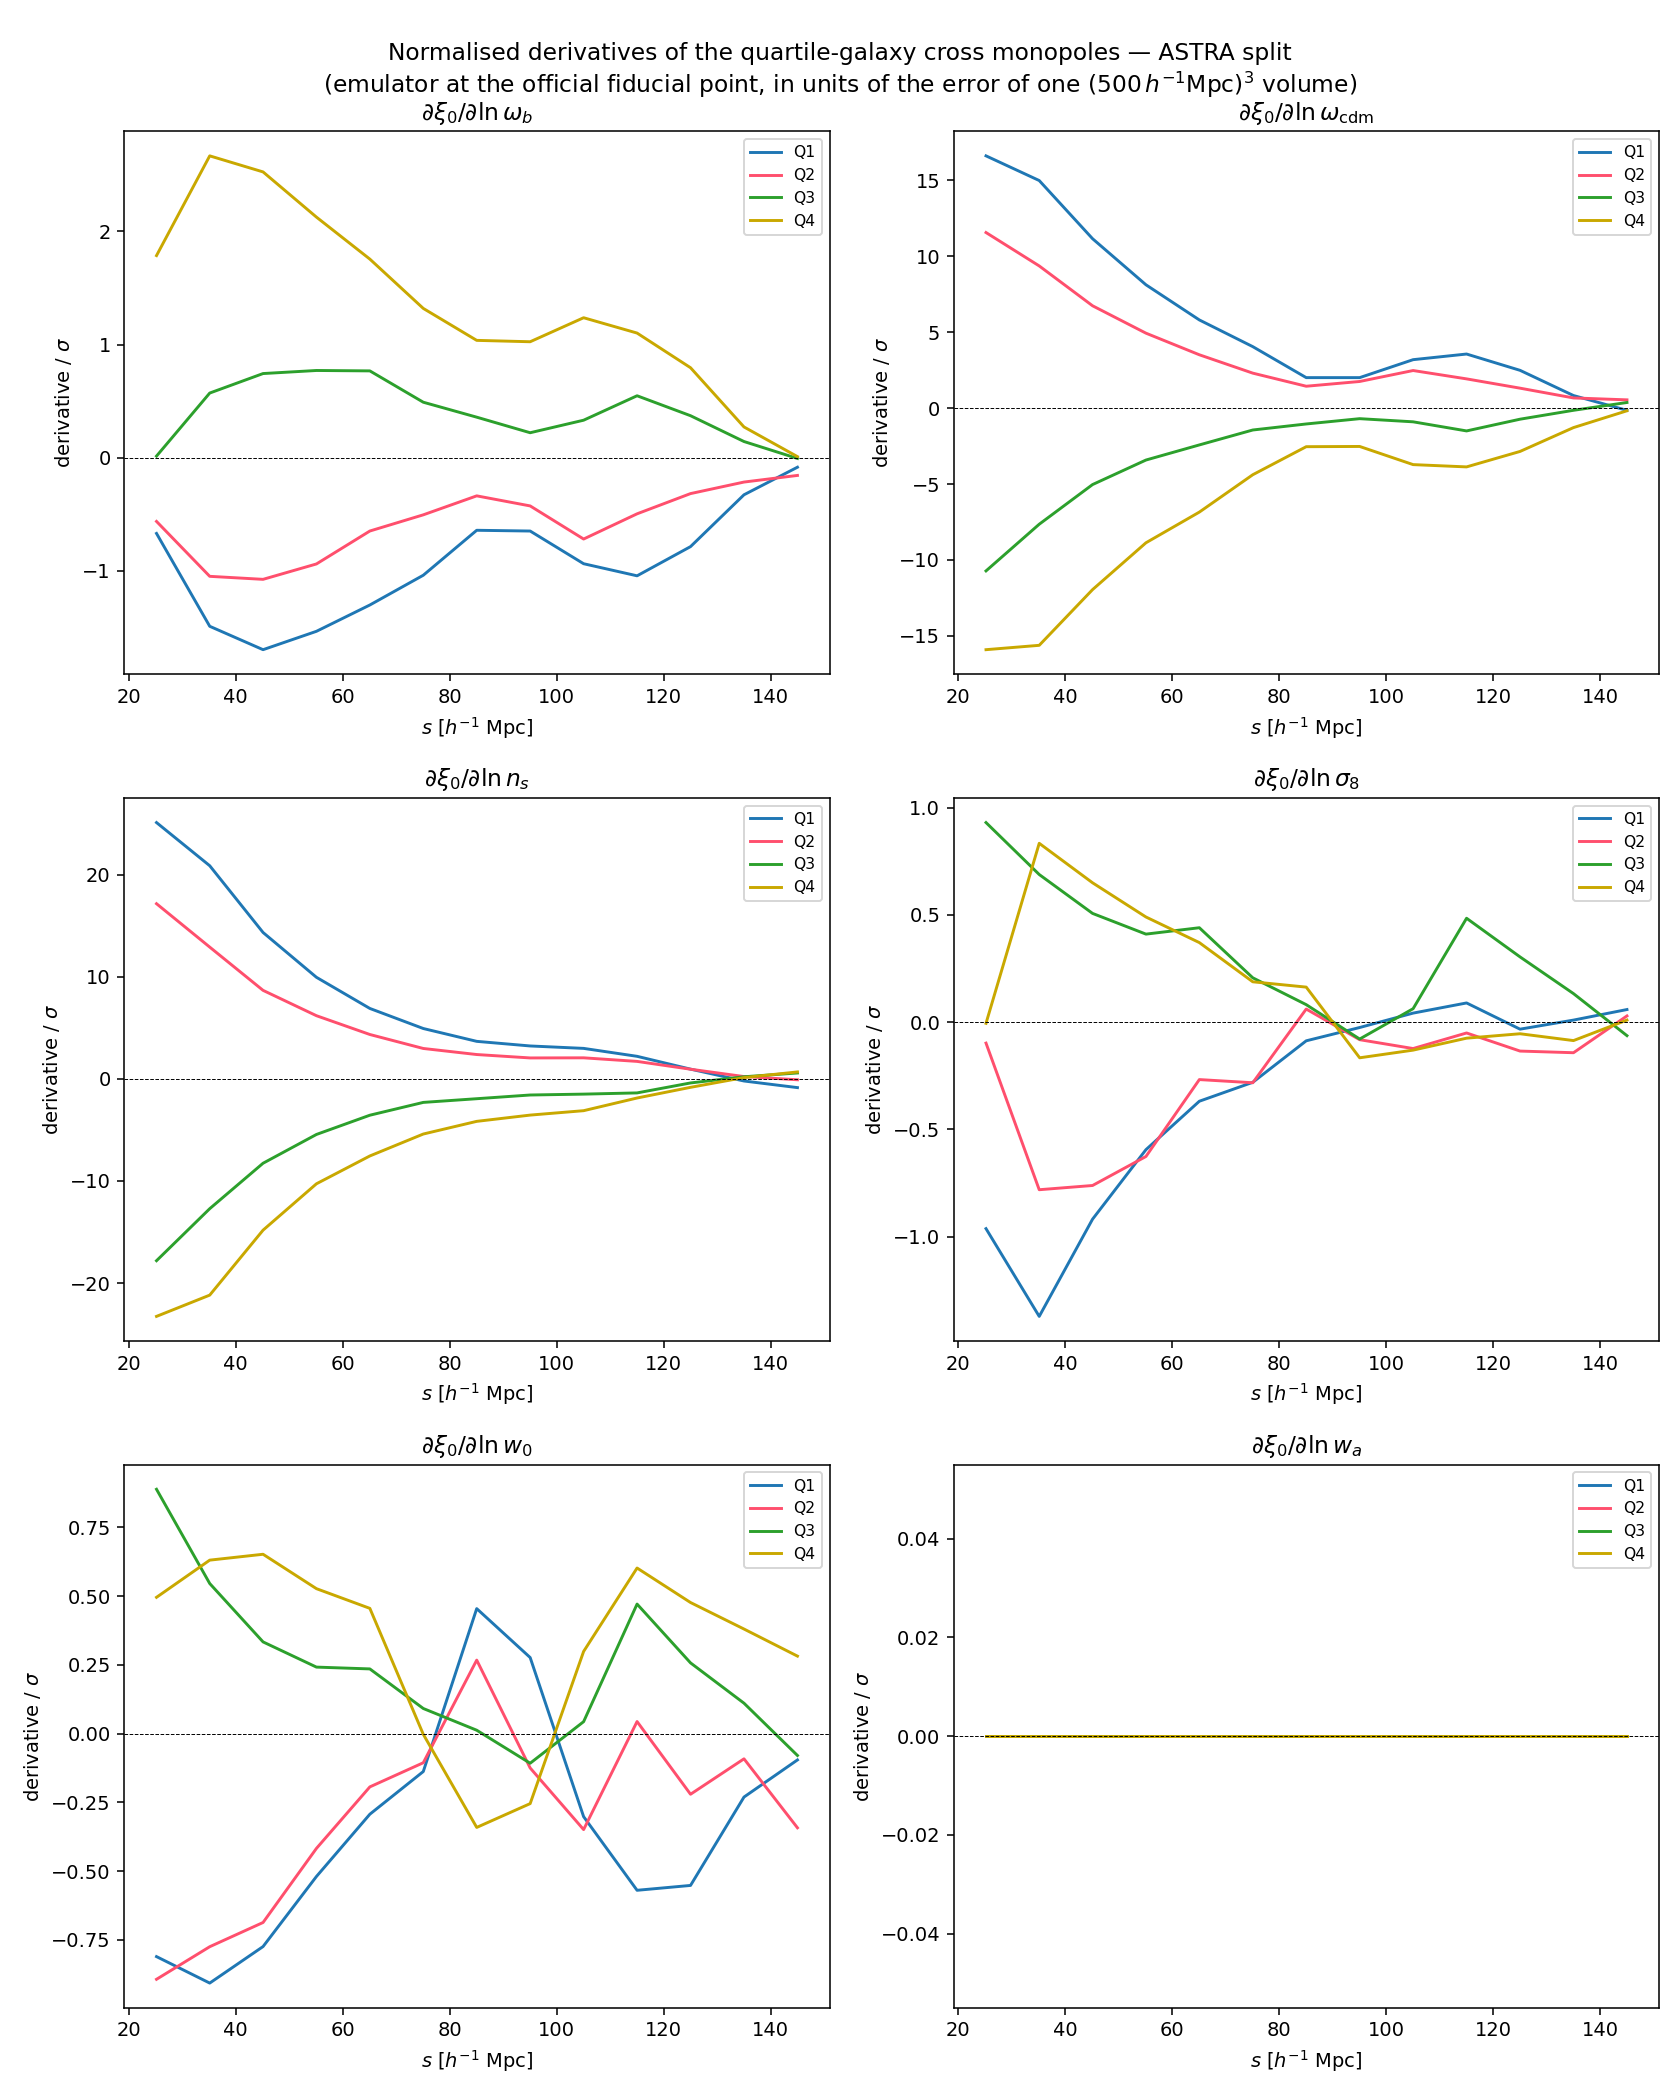
\includegraphics[width=\linewidth]{v1style_derivatives_astra.png}
\caption{ASTRA split: derivatives of the four quartile--galaxy cross monopoles with respect to the logarithm of each parameter, in units of the error of one $(500\Mpch)^3$ volume (baseline emulator, official fiducial point).}
\label{fig:der_astra}
\end{figure}

\begin{figure}[!htbp]
\centering
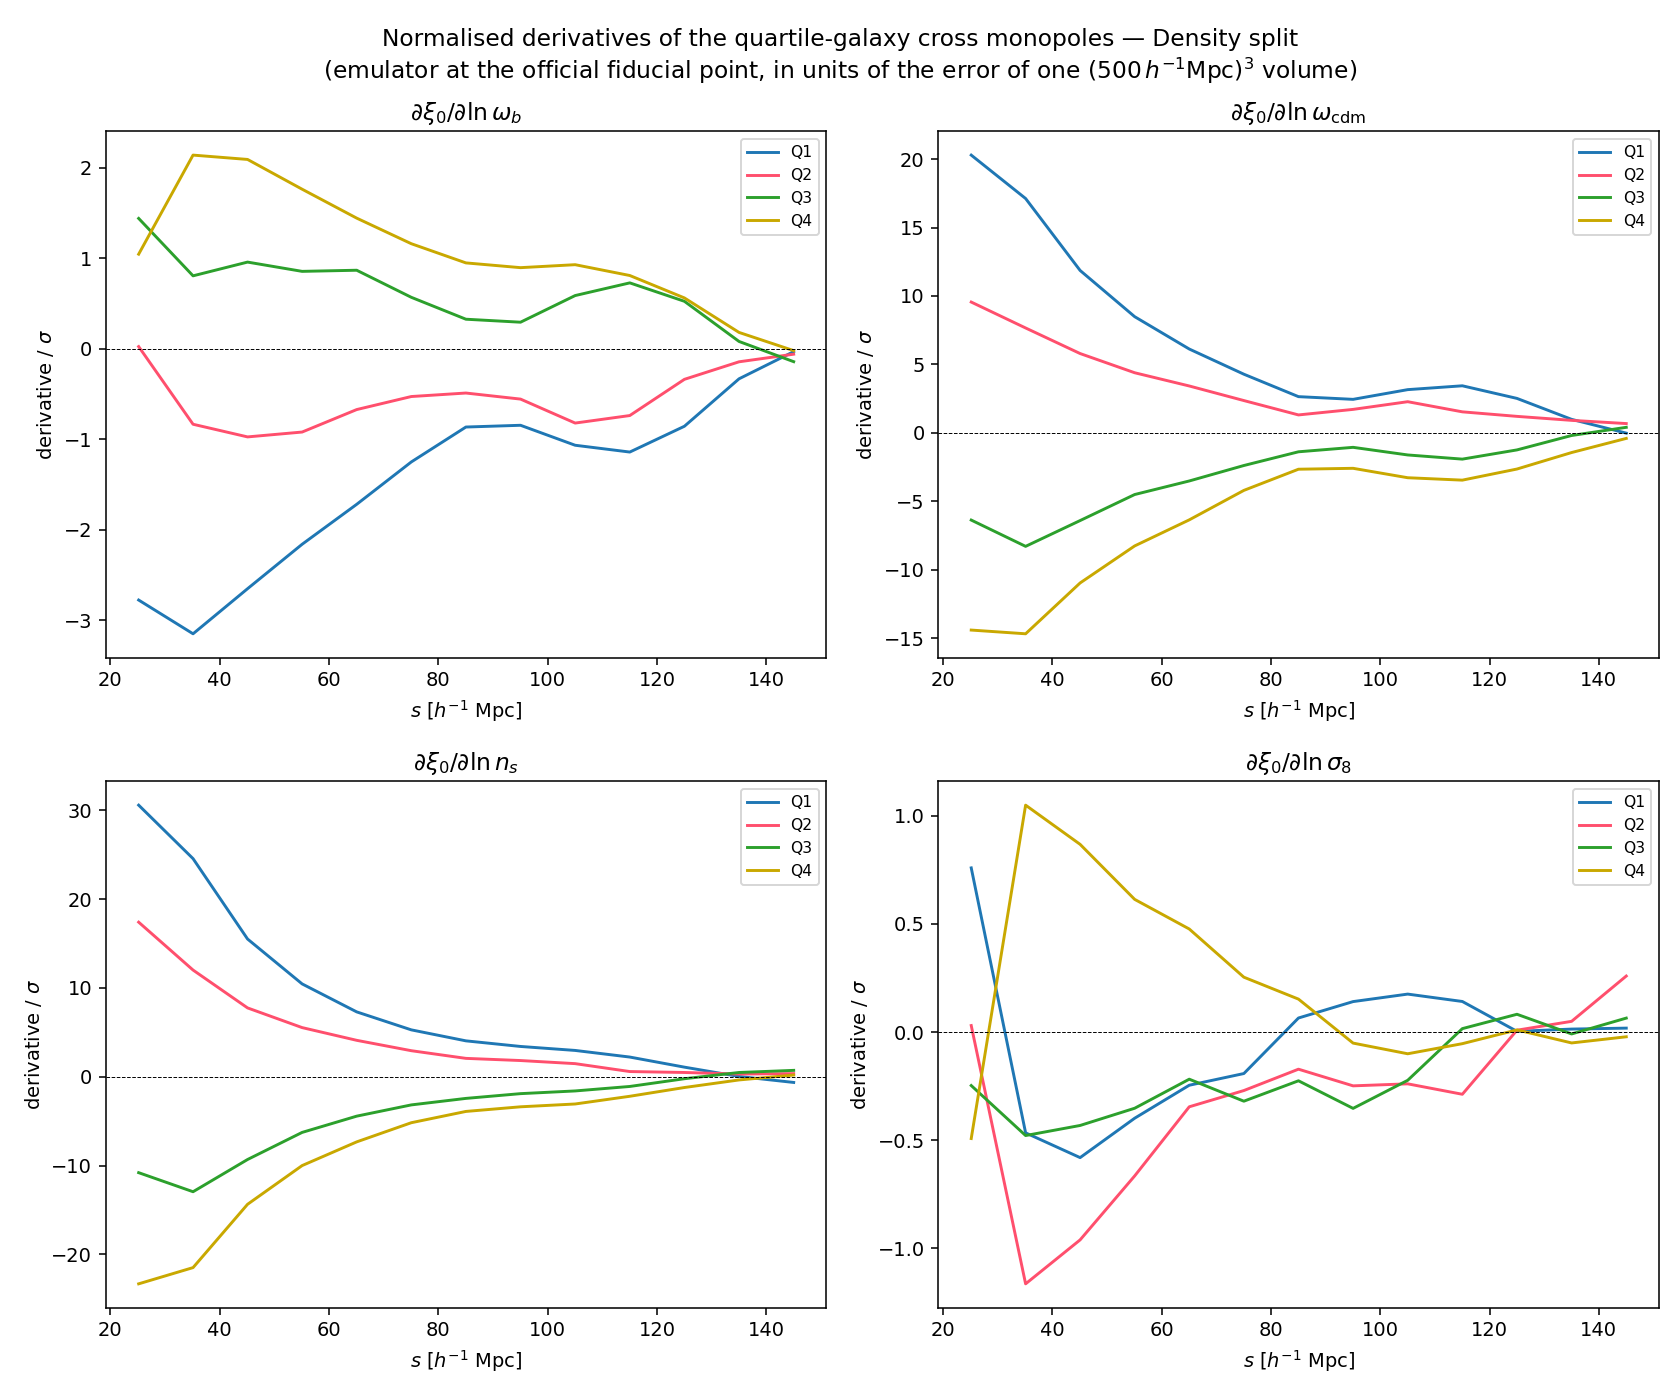
\includegraphics[width=\linewidth]{v1style_derivatives_ds.png}
\caption{Same as Figure~\ref{fig:der_astra} for density split.}
\label{fig:der_ds}
\end{figure}

\subsection{Derivatives from a regression over pairs}
\label{sec:regression}

As an alternative to the emulator, we estimate the derivatives locally from the derivative grid alone. For a pair of cosmologies $c_\pm$, all the catalogues of each cosmology within a distance $r_{\max}$ of the fiducial HOD $h_0$ (the 16 draws of the densification, the pair draw and the emulator draws) are fitted with a first-order expansion in the HOD parameters, $\boldsymbol d_c(h) = \boldsymbol a_c + G\,(h-h_0)$, with a response $G$ shared by the two cosmologies; the derivative is $(\boldsymbol a_{c_+}-\boldsymbol a_{c_-})/(\theta_+-\theta_-)$, the difference between the two cosmologies at exactly the fiducial HOD. The fit is performed subvolume by subvolume, so that part of the cosmic variance cancels, and the errors are obtained by bootstrapping the subvolumes. The intercepts are interpolated in the middle of draws surrounding $h_0$, and curvature common to the two cosmologies cancels in the difference. This estimator relies on a linear model and on the derivative grid only, while the emulator is a non-linear model of the whole suite: agreement between the two is a strong test of the derivatives.

\paragraph{Reduced HOD space.} With 12 HOD parameters and $\sim18$ catalogues per cosmology, the fit is poorly conditioned: its leave-one-out error is 0.8--1.0 times the scatter between HODs, and separate responses $G_\pm$ or quadratic terms do not help. We therefore restrict it to the most important directions of the HOD space, determined independently from the 72 fiducial calibration catalogues: the right singular vectors of the linear HOD response, each weighted by its statistical error. The singular values are $1, 0.054, 0.014, 0.013,\dots$: \emph{the clustering statistics respond essentially to a single combination of the 12 HOD parameters}, plausibly the large-scale galaxy bias. Keeping 3 or 4 directions, the leave-one-out error drops to 0.7--0.9 times the HOD scatter, at the level of the measurement noise, and the two choices give the same forecasts within 5\%. We use 3 directions.

\subsection{Fisher matrices}
\label{sec:fishermat}

The derivatives $D=\partial\boldsymbol d/\partial(\boldsymbol\theta,\boldsymbol h)$ are obtained at the fiducial point for the 6 cosmological parameters $\boldsymbol\theta=(\omega_b,\omega_{\rm cdm},n_s,\sigma_8,w_0,w_a)$ and the 12 HOD parameters $\boldsymbol h$. The covariance is the sum of the measured covariance and of the (diagonal) emulator error. The Fisher matrix $F = D^T\hat C^{-1}D + P_h$ includes a Gaussian prior $P_h$ on the HOD parameters of width 0.29 times the prior range (the standard deviation of the uniform prior); the cosmological errors are marginalised over the HOD by inverting the full $18\times18$ matrix, and we also quote errors at fixed HOD. Marginalising over the HOD degrades the constraints by less than $\sim30\%$, the most affected parameter being $n_s$. The uncertainty due to the emulator training is estimated from the scatter of the forecasts of the individual networks, divided by $\sqrt{10}$.

\paragraph{Compression.} Each data vector is compressed to one number per parameter (18 numbers), $\boldsymbol t=W^T\boldsymbol d$, $W=\tilde C^{-1}D$ ($\tilde C$: Ledoit--Wolf shrinkage estimate of the covariance), whose covariance is then estimated from the samples (Hartlap factor 0.91 with 192 samples, 0.99 with 1786). The compression is lossless if $\tilde C=C$ and otherwise loses information without biasing the forecast; it allows long and combined data vectors to be compared fairly.


